\documentclass[a4paper,12pt]{article}
\usepackage{amsmath}
\usepackage{listings}
\usepackage{xcolor}
\usepackage{float}
\usepackage{graphicx}
\usepackage{hyperref}



\lstset{
    language=Python,
    basicstyle=\ttfamily\small,
    keywordstyle=\color{blue},
    stringstyle=\color{red},
    commentstyle=\color{green},
    showstringspaces=false,
    numbers=left,
    numberstyle=\tiny\color{gray},
    breaklines=true,
}

\title{Intro to Machine Learning Assignment}
\author{Ibrahim Mohamed \\ Student ID: 7790 \\}
\date{\today}

\begin{document}

% Cover Page
\maketitle
\section*{Note}
This assignment was written using LaTeX. The source code for the document and the code used in this assignment can be found in the following GitHub link:
\url{https://github.com/H1MAA/Intro-To-Machine-Assignments}

\thispagestyle{empty}
\newpage

% Section 1: Linear Algebra
\section{Linear Algebra}
\textbf{Question 1:}
Find the eigenvalues of the following matrix \( A \):
\[
A = \begin{bmatrix}
0 & 1 & 0 \\
0 & 0 & 1 \\
4 & -17 & 8
\end{bmatrix}
\]
Eigenvalues: \(\lambda_1, \lambda_2, \lambda_3\), can be found by solving the following equation:
\[
\det(A - \lambda I) = 0
\]

This gives us the following:
\[
\det\left( \begin{bmatrix}
-\lambda & 1 & 0 \\
0 & -\lambda & 1 \\
4 & -17 & 8 - \lambda
\end{bmatrix} \right)
\]
Selecting the first row and using cofactor expansion and selecting the first column, we get:
\begin{equation*}
\det(A - \lambda I) = -\lambda \cdot \det \begin{bmatrix}
    -\lambda & 1 \\
    -17 & 8 - \lambda
    \end{bmatrix}
    - 1 \cdot \det \begin{bmatrix}
    0 & 1 \\
    4 & 8 - \lambda
    \end{bmatrix}
    + 0 \cdot \det \begin{bmatrix}
    0 & -\lambda \\
    4 & -17
    \end{bmatrix}
\end{equation*}
Fist term of the equation is:
\[
-\lambda \cdot \det \begin{bmatrix}
    -\lambda & 1 \\
    -17 & 8 - \lambda
    \end{bmatrix} = -\lambda \cdot (-\lambda \cdot (8 - \lambda) - 1 \cdot -17)
\]
Simplifying the above equation, we get:
\[
-\lambda \cdot (-\lambda \cdot (8 - \lambda) - 1 \cdot -17) = \lambda^3 + 8\lambda^2 - 17\lambda
\]
Second term of the equation is:
\[
- 1 \cdot \det \begin{bmatrix}
    0 & 1 \\
    4 & 8 - \lambda
    \end{bmatrix} = -1 \cdot (0 \cdot (8 - \lambda) - 1 \cdot 4)
\]
Simplifying the above equation, we get:
\[
-1 \cdot (0 \cdot (8 - \lambda) - 1 \cdot 4) = 4
\]
The third term of the equation is 0, so we can ignore it. Therefore, the equation becomes:
\[
-\lambda^3 + 8\lambda^2 - 17\lambda + 4 = 0
\]
Factorize:\[(\lambda - 4)(\lambda^2 - 4\lambda + 1) = 0\]
Therefore, the eigenvalues are:
\[
\lambda_1 = 4, \quad \lambda_{2,3} = 2 \pm \sqrt{3}
\]

\newpage

% Section 2: Probability
\section{Probability}
\textbf{Question 2:}
Three persons A, B, and C have applied for a job in a private company. The chance of their selections is in the ratio 1:2:4. The probabilities that A, B, and C can introduce changes to improve the profits of the company are 0.8, 0.5, and 0.3, respectively. If the change does not take place, find the probability that it is due to the appointment of C.\\
\\\textbf{\textit{Given:}}
\begin{align*}
    P(A) &= \frac{1}{7}, \quad P(B) = \frac{2}{7}, \quad P(C) = \frac{4}{7} \\
    P(\text{Change} \mid A) &= 0.8, \quad P(\text{Change} \mid B) = 0.5, \quad P(\text{Change} \mid C) = 0.3
\end{align*}
\textbf{\textit{Find:}}
\[
\mathbf{P(C \mid \textbf{No Change})}
\]
From the question we can deduce that:
\[
P(\text{Change}) = P(A) \cdot P(\text{Change} \mid A) + P(B) \cdot P(\text{Change} \mid B) + P(C) \cdot P(\text{Change} \mid C)
\]
\[
P(\text{Change}) = \frac{1}{7} \cdot 0.8 + \frac{2}{7} \cdot 0.5 + \frac{4}{7} \cdot 0.3 = \frac{3}{7}
\]
Therefore,
\[
P(\text{No Change}) = 1 - P(\text{Change}) = \frac{4}{7}
\]
And
\[
P(\text{No Change} \mid C) = 1 - P(\text{Change} \mid C) = 0.7
\]
We can get the probability of no change due to the appointment of C:
\[
P(C \mid \text{No Change}) = \frac{P(C) \cdot P(\text{No Change} \mid C)}{P(\text{No Change})}
\]
\[
P(C \mid \text{No Change}) = \frac{\frac{4}{7} \cdot 0.7}{\frac{4}{7}} = 0.7
\]
\newpage

% Section 3: K-Nearest Neighbor (KNN)
\section{K-Nearest Neighbor (KNN)}

\textbf{Question 3a:} Knowing that passed exam is the class label, predict the class of the following students using K-Nearest Neighbor for \( K = 3 \).\\

\textbf{Solution:}
We Can use the Euclidean distance to find the nearest neighbors. The Euclidean distance between two points \( (x_1, y_1) \) and \( (x_2, y_2) \) is given by:
\[
d = \sqrt{(x_2 - x_1)^2 + (y_2 - y_1)^2}
\]
Using python we can implement the Euclidean distance and the K-Nearest Neighbor algorithm as follows:
\begin{figure}[H]
    \centering
    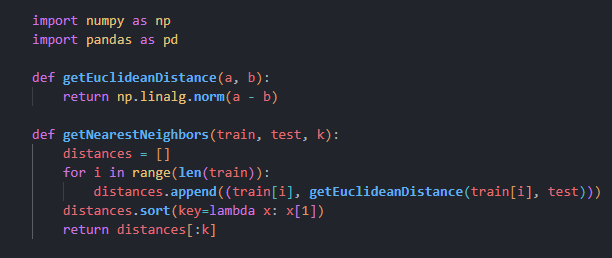
\includegraphics[width=0.9\textwidth]{knn.png}
    \caption{Euclidean Distance and Nearest Neighbors Functions}
    \label{fig:knn_code_example}
\end{figure}
\begin{figure}[H]
    \centering
    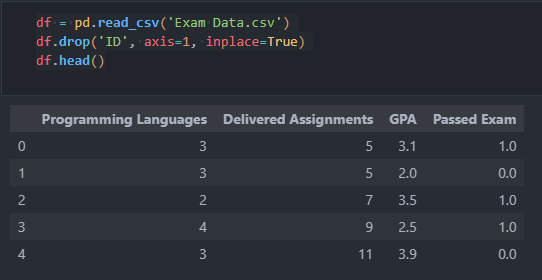
\includegraphics[width=0.8\textwidth]{data.png}
    \caption{Load data as a CSV file}
    \label{fig:dataframe_example}
\end{figure}
Then we can use the getNearestNeighbors function to find the nearest neighbors:
\begin{figure}[H]
    \centering
    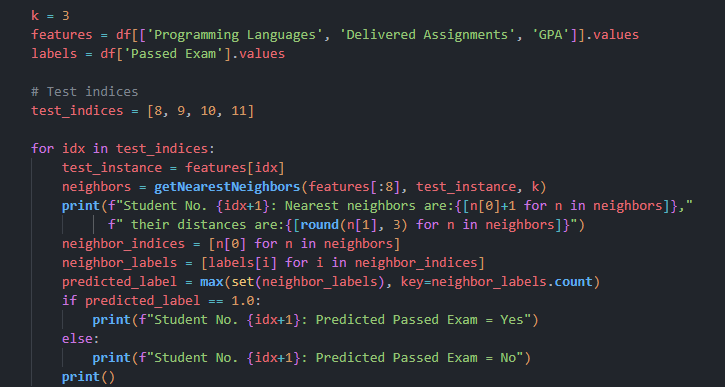
\includegraphics[width=1\textwidth]{getNeighbours.png}
    \caption{K-Nearest Neighbor Example}
    \label{fig:knn_example}
\end{figure}
\textbf{Results:}
\begin{itemize}
    \item \textbf{Student No. 9:}
    \begin{itemize}
        \item Nearest neighbors: [6, 7, 1], Distances: [1.005, 1.792, 3.164]
        \item Predicted Passed Exam: \textbf{No}
    \end{itemize}
    \item \textbf{Student No. 10:}
    \begin{itemize}
        \item Nearest neighbors: [6, 7, 1], Distances: [1.487, 2.1, 2.193]
        \item Predicted Passed Exam: \textbf{No}
    \end{itemize}
    \item \textbf{Student No. 11:}
    \begin{itemize}
        \item Nearest neighbors: [2, 1, 3], Distances: [1.414, 1.792, 2.693]
        \item Predicted Passed Exam: \textbf{Yes}
    \end{itemize}
    \item \textbf{Student No. 12:}
    \begin{itemize}
        \item Nearest neighbors: [1, 2, 3], Distances: [1.077, 1.803, 2.0]
        \item Predicted Passed Exam: \textbf{Yes}
    \end{itemize}
\end{itemize}
\newpage
\textbf{Question 3b:} Show the effect of feature scaling by transforming each feature (column) to be in the range \([0,1]\). The minimum value of the feature in the training data maps to 0, and the maximum value of the same feature maps to 1. Predict the labels again.\\
\textbf{Solution:}

to Scale the value of the features to be in the range \([0,1]\), we can use the Min-Max scaling method. The formula for Min-Max scaling is given by:
\begin{verbatim}
def minMaxScaler(data, scaler):
return (data - scaler.min()) / (scaler.max() - scaler.min())
\end{verbatim}
Giving Us the following results:
\begin{figure}[H]
    \centering
    \begin{minipage}{0.4\textwidth}
        \centering
        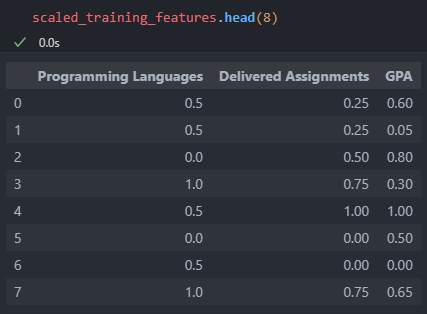
\includegraphics[width=\textwidth]{minmax0.png}
        \caption{Training}
        \label{fig:MinMax_training}
    \end{minipage}\hfill
    \begin{minipage}{0.55\textwidth}
        \centering
        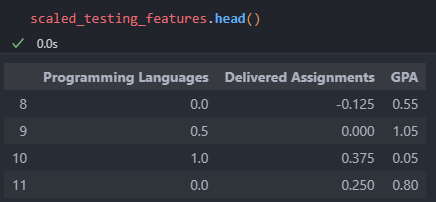
\includegraphics[width=\textwidth]{minmax1.png}
        \caption{Testing}
        \label{fig:MinMax_testing}
    \end{minipage}
\end{figure}
\textbf{Results:}
\begin{itemize}
    \item \textbf{Student No. 9:}
    \begin{itemize}
        \item Nearest neighbors: [6, 1, 3], Distances: [0.135, 0.627, 0.673]
        \item Predicted Passed Exam: \textbf{Yes}
    \end{itemize}
    \item \textbf{Student No. 10:}
    \begin{itemize}
        \item Nearest neighbors: [1, 6, 3], Distances: [0.515, 0.743, 0.75]
        \item Predicted Passed Exam: \textbf{Yes}
    \end{itemize}
    \item \textbf{Student No. 11:}
    \begin{itemize}
        \item Nearest neighbors: [4, 2, 7], Distances: [0.451, 0.515, 0.627]
        \item Predicted Passed Exam: \textbf{No}
    \end{itemize}
    \item \textbf{Student No. 12:}
    \begin{itemize}
        \item Nearest neighbors: [3, 6, 1], Distances: [0.25, 0.391, 0.539]
        \item Predicted Passed Exam: \textbf{Yes}
    \end{itemize}
\end{itemize}
\newpage

\textbf{Question 4:} 
Consider the set of training examples in the diagram below.

\begin{enumerate}
    \item How will the point (8, 8) be classified by the 1-nearest neighbor classifier?
    \begin{description}
        \item[Answer:] The point (8, 8) will be classified as Negative
        \end{description}
    \item How will the point (8, 1) be classified by the 1-nearest neighbor classifier?
    \begin{description}
        \item[Answer:] Similarly, the point (8, 1) will be classified as Positive 
        \end{description}
\end{enumerate}
\begin{figure}[H]
    \centering
    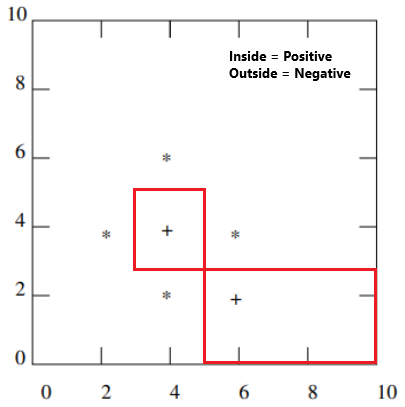
\includegraphics[width=1\textwidth]{q4.png}
    \caption{K-Nearest Neighbor Decision Boundary}
    \label{fig:knn_decision_boundary}
    
\end{figure}

\newpage

\textbf{Question 5:}
For the data given with 10 points and 2 classes:
\begin{enumerate}
    \item What is the leave-one-out cross-validation error when using K-nearest neighbor classifier with \( K = 1 \)?
    \item Which of the following values of K leads to the minimum number of leave-one-out validation errors: 3, 5, or 9?
\end{enumerate}
\textbf{Solution:}\\
From the given data, we can deduce that the shortest distance K = 1 for each point is of a different class. 
Therefore, the MSE for each point is 1. .\\
The leave one out cross-validation error can be calculated as follows:
\[
\text{Leave-One-Out Error} = \frac{1}{N} \sum_{i=1}^{N} \text{MSE}_i
\]
Therefore, the leave-one-out cross-validation error is 1.\\
he following values of K leads to the minimum number of leave-one-out validation errors is 5
\end{document}
